% !TEX root = ../tjumain.tex

\chapter{连接建立的设计}
该部分涉及到的TCP的状态转变如下图\ref{fig:fsm}所示:

\section{状态机设计}

TCP 可靠数据传输过程如下所示,对于出现丢包的情况,在 Client 端采用重传机制,不在 Server 端关于 ACK 丢掉的处理机制。同时,在 Server 端采用了 AVL Tree 的数据结构存储乱序到达的数据包,确保最终呈现在接收缓冲区的内容是有序的。

\subsection{Client 端状态机设计}

\begin{figure}[!htbp]
    \centering
    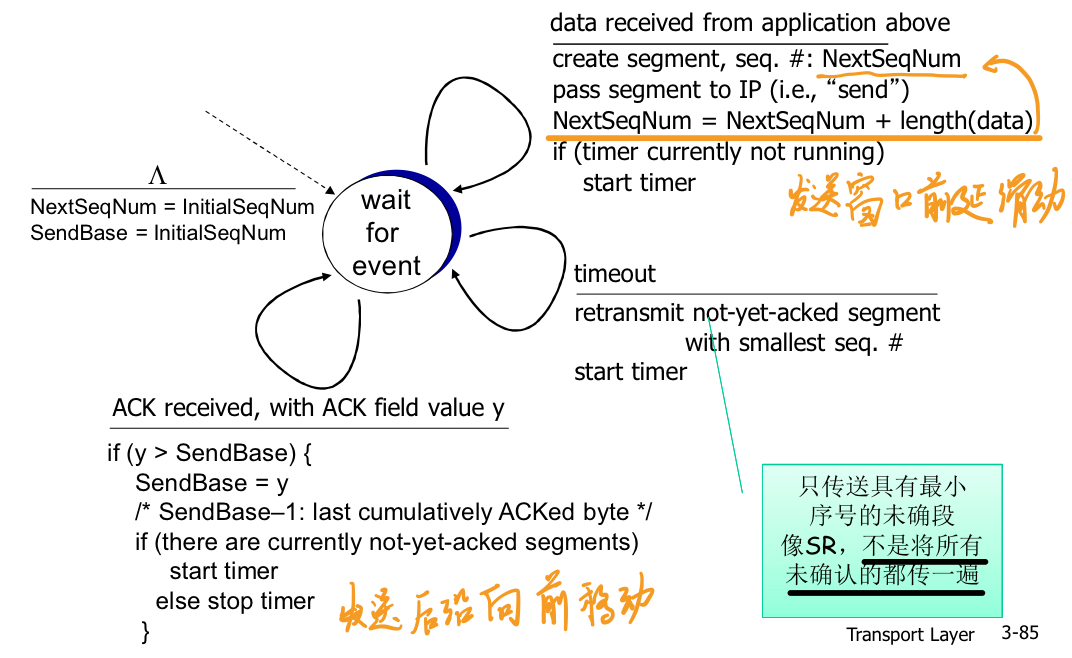
\includegraphics[width=.8\textwidth]{figures/CLIENT_FSM.png}
    \label{fig:client_fsm}\caption{Client FSM}
  \end{figure}

Client 端状态机如图\ref{fid:client_fsm}所示。Client 端需要响应三种事件:
\begin{enumerate}
    \item 来自上层的调用,将数据打包并发送给下一层实体(toLayer3),然后新建 TIMER 并 注册之
    \item 来自TIMEOUT 通过 TIMER 的信息进行超时重传(需要调整一下rtt等信息)
    \item 收到 ACK,确认 ACK 的状态,根据 ACK 信息选择性地关闭 TIMER 
\end{enumerate}

\subsection{Server 端状态机设计}

\begin{figure}[!htbp]
    \centering
    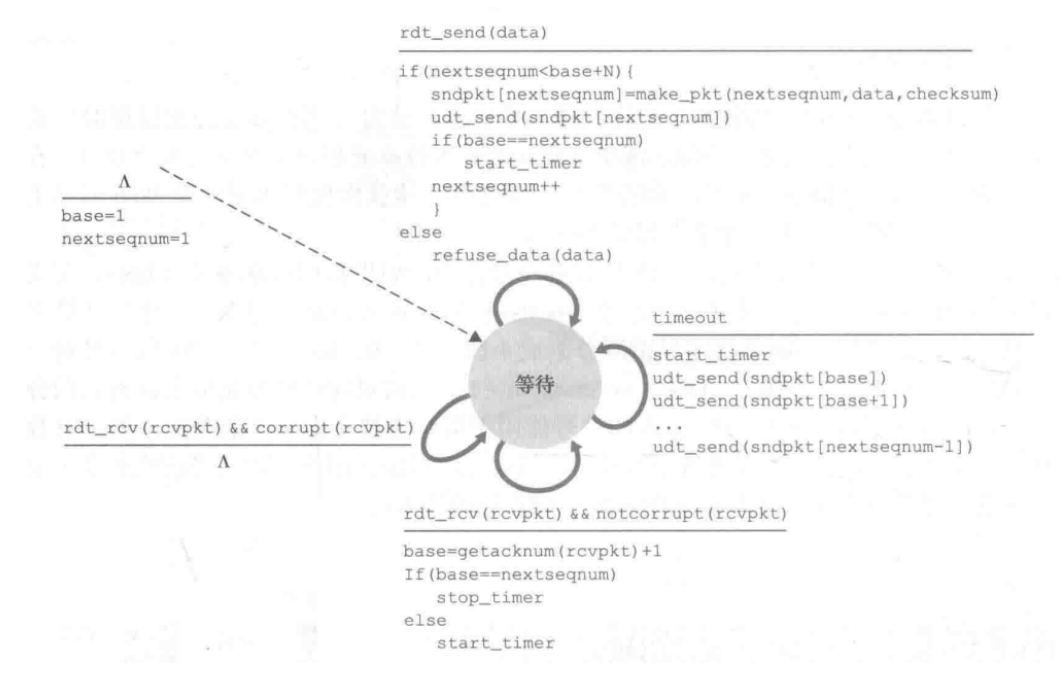
\includegraphics[width=.8\textwidth]{figures/SERVER_FSM.png}
    \label{fig:server_fsm}\caption{Server FSM}
  \end{figure}

在 Server 端,我们目前暂不考虑数据出错的情况,即达到的包,都是正确的。在此情况下,我们需要处理一下情况:


\begin{enumerate}
    \item 到达SEQ正确:判断缓冲区大小,选择性的将其放入缓冲区,发送ACK。同时在AVL中递归地查找连续的正确的包裹
    \item 到达SEQ大了:将其放入 AVL Tree 并发送ACK
    \item 到达SEQ小了:收到过,丢弃
\end{enumerate}

\section{超时重传机制}

\paragraph*{连接建立时} 丢失有三种:第一次握手丢失,服务端返回第二次握手丢失,以及第三次确认丢失。第一、二个由 Client 端设置定时器保护,第三个由 Server 端设置定时器保护,即当收到第三次确认时,Server 端再将信息定时器进行关闭。

\paragraph*{发送数据时} 丢失有两种:发送数据丢失(Seq),发送ACK丢失。二者对于 Client 端的表现均是长时间(RTO)没收到 ACK 信息,于是我们将定时器设置在 Client 端,由 Client 端进行超时重传。而 Server 只对于前者,即发送数据丢失的情况作出反馈,即设置乱序到达,顺序提交的机制,确保因超时而呈现乱序到达的数据得以顺序提交给上层用户。

\section{RTO 计算法则}

RTO 是超时重传机制的基础。由于网络变化,RTO应当是动态调整的。如果TCP 过早重传,会导致注入多数不必要的报文,阻塞网络。如果过晚重传,则会影响网络使用效率。我们根据 RFC793 的标准,让Socket维护了一个 SampleRTT均值(EstimatedRTT)通过如下公式进行更新:
\begin{equation}
    EstimatedRTT := (1-\alpha)\times EstimatedRTT + \alpha\times SampleRTT
\end{equation}\label{eq:est}

除了RTT,RFC 6298 还定义了 RTT 的偏差 DevRTT 的计算,用于usuan SampleRTT 和EstimatedRTT 的偏离程度
\begin{equation}
    DevRTT := (1-\beta)\times DevRTT + \beta\times|SampleRTT - EstimatedRTT|
\end{equation}
于是,最终的TRO计算公式如下:
\begin{equation}
    RTO := EstimatedRTT + 4\times DevRTT
\end{equation}\label{eq:rto}

\section{流量控制}

流量控制也是 TCP 标准功能之一,是构成可靠传输的关键步骤,能够与其他 TCP 实体一起,维护整个网络的传输可靠性。如果流量过大,则会导致接收方不断丢弃传输的结果,发送方不断进行重发。故而,Server 端需要将rwnd的信息通过 ACK 信息携带给 Client 端,让 Client 能够正确地调整发送速率。
